
\subsubsection{Module MD-09: Quản lý Phiên \& Báo cáo}

Module Quản lý Phiên \& Báo cáo (MD-09) là một thành phần thiết yếu trong hệ thống quản lý nhà hàng, tập trung vào việc cung cấp các công cụ để theo dõi, tổng kết và phân tích hoạt động bán hàng từ các phiên làm việc Point of Sale (POS). Module này cho phép Quản lý nhà hàng và Kế toán truy cập vào dữ liệu lịch sử, xem xét hiệu suất kinh doanh, đối soát tài chính, và đưa ra các quyết định dựa trên số liệu thực tế.




\begin{figure}[H]
    \centering
    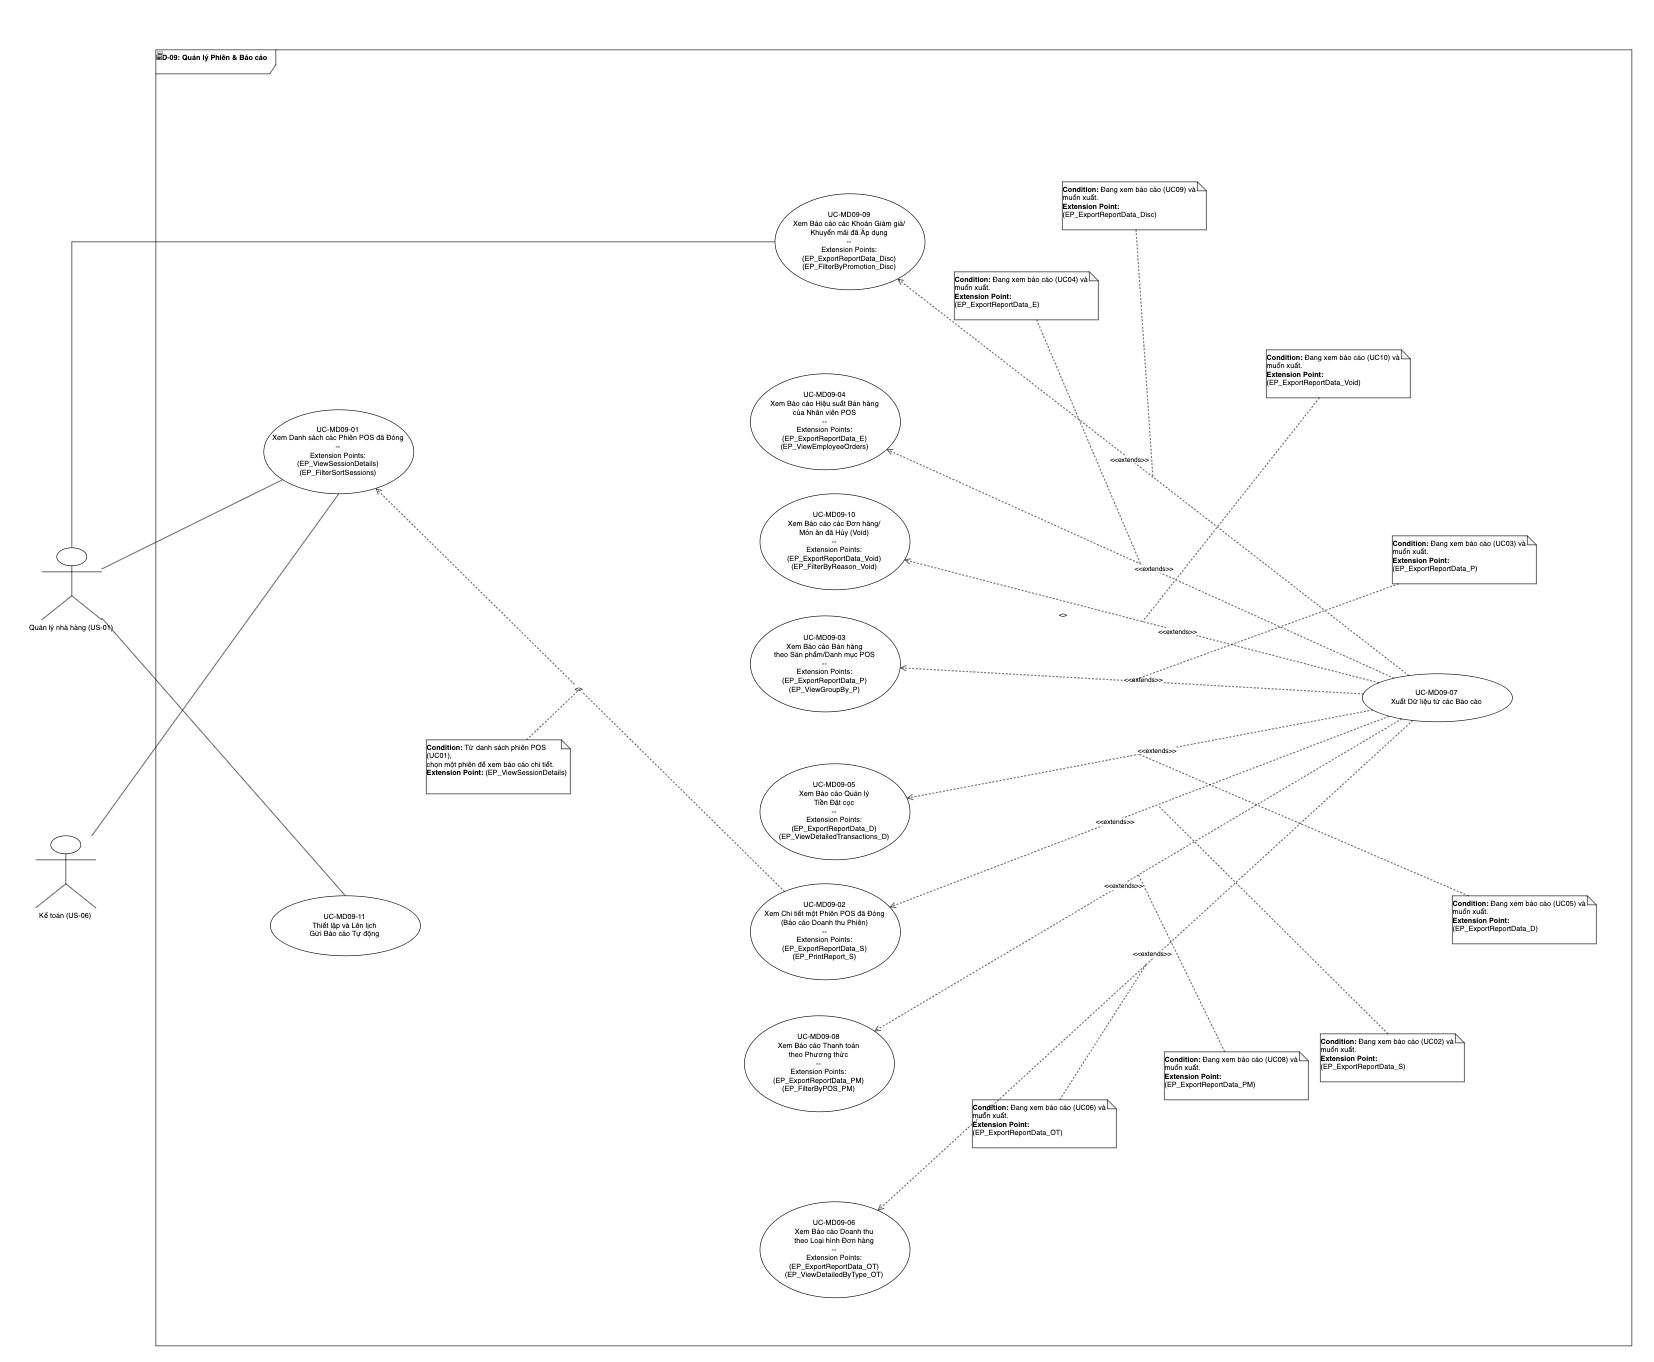
\includegraphics[width=15cm]{Sections/tong_quan/functional_spec/img/uc9.png}
    \vspace{0.5cm}
    \caption{Use case diagram cho Module MD-09}
    \label{fig:my_label}
\end{figure}

\begin{longtable}{|m{2cm}|m{2.5cm}|m{2cm}|m{4.5cm}|m{4cm}|}
\caption{Danh sách Yêu cầu Chức năng cho Module MD-09: Quản lý Phiên \& Báo cáo} \label{tab:fr_md09_revised_v2} \\
\hline
\textbf{Mã Module} & \textbf{Mã Yêu cầu CN} & \textbf{Mã Người dùng} & \textbf{Tên Chức năng} & \textbf{Mô tả Ngắn} \\
\hline
\endhead % Header cho các trang tiếp theo
\hline
\endfoot % Footer cho bảng
\hline
\endlastfoot % Footer cho trang cuối cùng

MD-09 & FR-MD09-01 & US-01/US-06 & Xem Danh sách các Phiên POS đã Đóng & Cho phép Quản lý/Kế toán xem danh sách các phiên POS đã được đóng. \\
\hline
MD-09 & FR-MD09-02 & US-01/US-06 & Xem Chi tiết một Phiên POS đã Đóng (Báo cáo Doanh thu Phiên) & Cung cấp báo cáo chi tiết về doanh thu, thanh toán, tiền mặt... của một phiên POS cụ thể đã đóng. \\
\hline
MD-09 & FR-MD09-03 & US-01/US-06 & Xem Báo cáo Tổng hợp Bán hàng theo Sản phẩm/Danh mục POS & Thống kê số lượng và doanh thu của từng sản phẩm/danh mục POS trong một khoảng thời gian. \\
\hline
MD-09 & FR-MD09-04 & US-01 & Xem Báo cáo Hiệu suất Bán hàng của Nhân viên POS & Thống kê doanh thu hoặc số lượng đơn hàng do từng nhân viên xử lý trên POS. \\
\hline
MD-09 & FR-MD09-05 & US-01/US-06 & Xem Báo cáo Quản lý Tiền Đặt cọc & Báo cáo tổng hợp tình hình thu, sử dụng, và mất cọc từ các lượt đặt chỗ. \\
\hline
MD-09 & FR-MD09-06 & US-01/US-06 & Xem Báo cáo Doanh thu theo Loại hình Đơn hàng & Phân tích doanh thu dựa trên các loại hình: Ăn tại chỗ, Mang về, Giao hàng. \\
\hline
MD-09 & FR-MD09-07 & US-01/US-06 & Xuất Dữ liệu từ các Báo cáo & Cho phép xuất dữ liệu báo cáo ra định dạng Excel/CSV. \\
\hline
MD-09 & FR-MD09-08 & US-01/US-06 & Xem Báo cáo Thanh toán theo Phương thức & Thống kê tổng số tiền thu được theo từng phương thức thanh toán (Tiền mặt, Ví điện tử...) trong một khoảng thời gian. \\
\hline
MD-09 & FR-MD09-09 & US-01 & Xem Báo cáo các Khoản Giảm giá/Khuyến mãi đã Áp dụng & Thống kê tổng giá trị giảm giá đã được áp dụng trên các đơn hàng trong một khoảng thời gian. \\
\hline
MD-09 & FR-MD09-10 & US-01 & Xem Báo cáo các Đơn hàng/Món ăn đã Hủy (Void) & Thống kê số lượng và giá trị các đơn hàng hoặc món ăn đã bị hủy trên POS, có thể kèm lý do. \\
\hline
MD-09 & FR-MD09-11 & US-01/US-06 & (Tùy chọn) Thiết lập và Lên lịch Gửi Báo cáo Tự động & Cho phép cấu hình để hệ thống tự động gửi một số báo cáo nhất định (ví dụ: báo cáo doanh thu ngày) đến email của người quản lý theo lịch. \\
\hline

\end{longtable}

\subsubsubsection{Mục tiêu và Phạm vi}
\label{sssec:md08_objectives_scope}
Mục tiêu chính của module MD-08 là:
\begin{itemize}
    \item \textbf{Truyền tải chính xác yêu cầu món ăn:} Đảm bảo mọi chi tiết của đơn hàng (tên món, số lượng, biến thể, ghi chú đặc biệt) được gửi từ POS đến bếp một cách đầy đủ và không sai sót.
    \item \textbf{Tối ưu hóa quy trình làm việc trong bếp:} Giúp nhân viên bếp dễ dàng tiếp nhận, xem, quản lý và theo dõi tiến độ chuẩn bị các món ăn.
    \item \textbf{Giảm thiểu sai sót và nhầm lẫn:} Hạn chế việc trao đổi thông tin bằng miệng hoặc giấy tờ dễ thất lạc, từ đó giảm lỗi trong quá trình chế biến.
    \item \textbf{Cải thiện thời gian phục vụ:} Giúp bếp nhận yêu cầu nhanh hơn và quản lý thứ tự ưu tiên hiệu quả hơn (đặc biệt với KDS).
    \item \textbf{(Nếu dùng KDS) Cung cấp khả năng theo dõi và cập nhật trạng thái:} Cho phép nhân viên bếp đánh dấu trạng thái chế biến (đang làm, đã xong) và (tùy chọn) đồng bộ thông tin này ngược lại cho nhân viên phục vụ.
    \item \textbf{Hỗ trợ định tuyến thông minh:} Đảm bảo các món ăn được gửi đến đúng trạm chuẩn bị (ví dụ: món chính gửi bếp chính, đồ uống gửi quầy bar) nếu nhà hàng có nhiều khu vực bếp/bar.
\end{itemize}

\subsubsubsection{Mục tiêu và Phạm vi}
\label{sssec:md09_objectives_scope}
Mục tiêu chính của module MD-09 là:
\begin{itemize}
    \item \textbf{Cung cấp thông tin tổng kết phiên POS:} Cho phép xem lại chi tiết tài chính và hoạt động của từng phiên POS đã đóng.
    \item \textbf{Phân tích hiệu quả bán hàng:} Cung cấp các báo cáo đa dạng về doanh thu theo sản phẩm, danh mục, nhân viên, và loại hình đơn hàng.
    \item \textbf{Hỗ trợ đối soát tài chính:} Cung cấp báo cáo về các phương thức thanh toán và quản lý tiền đặt cọc, giúp kế toán dễ dàng đối soát.
    \item \textbf{Kiểm soát thất thoát và hoạt động bất thường:} Thông qua báo cáo về các đơn hàng/món ăn đã hủy.
    \item \textbf{Tăng cường khả năng ra quyết định dựa trên dữ liệu:} Cung cấp thông tin đầu vào quan trọng cho việc lập kế hoạch kinh doanh, marketing, và quản lý nhân sự.
    \item \textbf{(Tùy chọn) Tự động hóa việc gửi báo cáo:} Giúp các nhà quản lý nhận được thông tin quan trọng một cách định kỳ mà không cần thao tác thủ công.
\end{itemize}
Phạm vi của module bao gồm việc hiển thị danh sách các phiên POS đã đóng, cung cấp báo cáo chi tiết cho từng phiên, tạo các báo cáo tổng hợp và phân tích về doanh thu, sản phẩm, nhân viên, thanh toán, giảm giá, hủy đơn, và (tùy chọn) thiết lập cơ chế gửi báo cáo tự động. Dữ liệu đầu vào cho module này chủ yếu đến từ các giao dịch được ghi nhận trong các module POS (MD-05, MD-06, MD-07) và Đặt chỗ (MD-03, liên quan đến đặt cọc).

\subsubsubsection{Đối tượng Sử dụng Chính}
\label{sssec:md09_primary_users}
Các đối tượng người dùng chính tương tác với module này bao gồm:
\begin{itemize}
    \item \textbf{US-01 (Quản lý nhà hàng):} Là người dùng thường xuyên nhất, sử dụng các báo cáo để theo dõi tình hình kinh doanh, đánh giá hiệu suất, kiểm soát hoạt động và đưa ra các quyết định chiến lược.
    \item \textbf{US-06 (Kế toán):} Sử dụng các báo cáo (đặc biệt là báo cáo chi tiết phiên, báo cáo thanh toán theo phương thức, báo cáo tiền đặt cọc) để thực hiện công việc đối soát tài chính, hạch toán kế toán.
\end{itemize}

\subsubsubsection{Các Chức năng Chính}
\label{sssec:md09_key_functionalities}
Module MD-09 cung cấp một loạt các chức năng báo cáo và quản lý dữ liệu lịch sử, được mô tả chi tiết qua các Use Case sau:

\begin{itemize}
    \item \textbf{Quản lý và Xem lại Phiên POS (UC-MD09-01, UC-MD09-02):}
    \begin{itemize}
        \item Cho phép xem danh sách các phiên làm việc POS đã được đóng, với các thông tin tóm tắt và khả năng lọc/tìm kiếm (UC-MD09-01).
        \item Xem báo cáo chi tiết tổng kết của một phiên POS cụ thể đã đóng, bao gồm doanh thu, chi tiết thanh toán, và đối chiếu tiền mặt (nếu có) (UC-MD09-02).
    \end{itemize}

    \item \textbf{Báo cáo Phân tích Bán hàng (UC-MD09-03, UC-MD09-04, UC-MD09-06, UC-MD09-08, UC-MD09-09, UC-MD09-10):}
    \begin{itemize}
        \item Xem báo cáo thống kê về số lượng bán ra và doanh thu của từng sản phẩm hoặc theo từng danh mục sản phẩm POS (UC-MD09-03).
        \item Xem báo cáo về hiệu suất bán hàng của từng nhân viên POS, bao gồm tổng doanh thu và số lượng đơn hàng (UC-MD09-04).
        \item Xem báo cáo phân tích tổng doanh thu theo từng loại hình đơn hàng (Ăn tại chỗ, Mang về, Giao hàng) (UC-MD09-06).
        \item Xem báo cáo thống kê tổng số tiền đã thu được qua từng phương thức thanh toán khác nhau (UC-MD09-08).
        \item Xem báo cáo về tổng giá trị các khoản giảm giá hoặc chương trình khuyến mãi đã được áp dụng (UC-MD09-09).
        \item Xem báo cáo thống kê về các món ăn hoặc toàn bộ đơn hàng đã bị hủy (voided) trên POS (UC-MD09-10).
    \end{itemize}

    \item \textbf{Báo cáo Quản lý Đặc thù (UC-MD09-05):}
    \begin{itemize}
        \item Xem báo cáo tổng hợp về tình hình thu và sử dụng tiền đặt cọc từ các lượt đặt chỗ (UC-MD09-05).
    \end{itemize}

    \item \textbf{Tiện ích Báo cáo (UC-MD09-07, UC-MD09-11):}
    \begin{itemize}
        \item Cho phép xuất dữ liệu từ các giao diện báo cáo ra các định dạng tệp phổ biến như Excel hoặc CSV (UC-MD09-07).
        \item (Tùy chọn) Cho phép thiết lập và lên lịch để hệ thống tự động tạo và gửi một số loại báo cáo nhất định đến email theo định kỳ (UC-MD09-11).
    \end{itemize}
\end{itemize}

\subsubsubsection{Tóm tắt Luồng Hoạt động Tổng thể}
\label{sssec:md09_overall_workflow}
Luồng hoạt động chính trong module Quản lý Phiên & Báo cáo thường diễn ra như sau:
\begin{enumerate}
    \item \textbf{Truy cập thông tin phiên đã đóng:}
        \begin{itemize}
            \item Người dùng (Quản lý/Kế toán) Xem Danh sách các Phiên POS đã Đóng (UC-MD09-01).
            \item Từ danh sách, người dùng chọn một phiên cụ thể để Xem Chi tiết một Phiên POS đã Đóng (Báo cáo Doanh thu Phiên) (UC-MD09-02).
        \end{itemize}
    \item \textbf{Xem các báo cáo phân tích và tổng hợp:}
        \begin{itemize}
            \item Người dùng lựa chọn và xem các loại báo cáo khác nhau tùy theo nhu cầu phân tích:
                \begin{itemize}
                    \item Báo cáo Tổng hợp Bán hàng theo Sản phẩm/Danh mục POS (UC-MD09-03).
                    \item Báo cáo Hiệu suất Bán hàng của Nhân viên POS (UC-MD09-04).
                    \item Báo cáo Quản lý Tiền Đặt cọc (UC-MD09-05).
                    \item Báo cáo Doanh thu theo Loại hình Đơn hàng (UC-MD09-06).
                    \item Báo cáo Thanh toán theo Phương thức (UC-MD09-08).
                    \item Báo cáo các Khoản Giảm giá/Khuyến mãi đã Áp dụng (UC-MD09-09).
                    \item Báo cáo các Đơn hàng/Món ăn đã Hủy (Void) (UC-MD09-10).
                \end{itemize}
            \item Trong quá trình xem các báo cáo này, người dùng có thể cần Xuất Dữ liệu từ các Báo cáo (UC-MD09-07) ra file để lưu trữ hoặc phân tích thêm.
        \end{itemize}
    \item \textbf{(Tùy chọn) Thiết lập gửi báo cáo tự động:}
        \begin{itemize}
            \item Nếu có nhu cầu, người dùng có thể Thiết lập và Lên lịch Gửi Báo cáo Tự động (UC-MD09-11) cho các báo cáo quan trọng.
        \end{itemize}
\end{enumerate}
Module MD-09 cung cấp cái nhìn sâu sắc về hoạt động kinh doanh của nhà hàng, hỗ trợ việc đưa ra các quyết định quản lý dựa trên dữ liệu chính xác và kịp thời, đồng thời đảm bảo tính minh bạch và kiểm soát tài chính.

